\documentclass[11pt]{article}
\usepackage[utf8]{inputenc}
\usepackage[T1]{fontenc}
\usepackage[spanish]{babel}
\usepackage{amsmath}
\usepackage{amsfonts}
\usepackage{amssymb}
\usepackage{graphicx}
\usepackage{caption}
\usepackage{wrapfig}
\usepackage{subcaption}
\usepackage{textcomp}
\usepackage{siunitx}
\usepackage{geometry}
\usepackage{courier}
\usepackage{cancel}
\usepackage{bm}
\spanishdecimal{.}

\title{Física Numérica}
\author{Julio César Avila Torreblanca}
\date{15 de diciembre del 2021}

\setlength{\parindent}{0cm}
\geometry{verbose,tmargin=1in,bmargin=1in,lmargin=1in,rmargin=1in}
\begin{document}
	\maketitle
	
	\section*{Tarea 8}
	%%%%%%%%%%%%%%%%%%%%%%%%%%%%%%%%%%%%%%%%%%%%%%%%%%%%%%%%%%%%%%%%%%%%%%%%%%%%%%%%%%%%%%%%%%%%%%%%%%%%%%%%%%%%%%%%%%%%%%%%	
	\subsection*{\textbf{Lanzamiento de martillo.}}
	El record mundial de martillo es de 86.74 m por Yuri Sedykh y se ha mantenido desde 1986. El martillo pesa 7.26 kg, es esférico, y tiene un radio de $R=6$ cm. La fricción en el martillo puede ser considerada proporcional al cuadrado de la velocidad del martillo relativa al aire:
	\begin{equation}
		F_D = \frac{1}{2} \rho A C_D v^2
	\end{equation}
	donde $\rho$ es la densidad del aire ($\SI{1.2}{kg/m^3}$) y $A=\pi R^2$ es la sección transversal del martillo. El martillo puede experimental, en principio, un flujo laminar con coeficiente de rozamiento $C_D=0.5$ o un flujo inestable osciante con coeficiente de rozamiento $C_D=0.75$.  
	\begin{enumerate}
		\item Resuelva la ecuación de movimiento para el lanzamiento oblicuo de martillo. Deberá transformar las EDOs para los movimientos en $x$ y $y$ en un sistema de cuatro ecuaciones de primer orden. Considere lanzamienos desde una posición inicial $x_0 = 0$ y $y_0 = \SI{2}{m}$, para un ángulo ideal $\phi = 45°$ y encuentre la velocidad que produce la distancia del lanzamiento del récord mundial.
	\end{enumerate}
\textit{Solución.}\\
	Sea $\bm{r} = (x,y)$ la posición del martillo. Luego, por la segunda ley de Newton tenemos la siguiente ecuación que describe el movimiento:
	\begin{eqnarray}
		m \bm{\ddot{r}} = \bm{F}_D + \bm{F}_g	\label{eq1}
	\end{eqnarray}
	Donde $\bm{F}_D$ es la fuerza de fricción y $\bm{F}_g$ es la fuerza gravitacional. Notemos que $\bm{F}_D$ debe tener sentido opuesto a la velocidad, para ello se debe multiplicar por un vector unitario en sentido opuesto a la velocidad, es decir:
	$$\bm{F}_D =  \frac{1}{2} \rho AC_D v^2 \left(-\frac{\bm{v}}{|\bm{v}|}\right)$$
	Donde $\bm{v} = (\dot{x}, \dot{y})$ y $v^2 = \dot{x}^2 +\dot{y}^2$.
	Por componentes se sigue que:
	\begin{align*}
		m\frac{d^2 x}{dt^2} &= \frac{1}{2}\rho A C_D (\dot{x}^2 + \dot{y}^2)\left(-\frac{\dot{x}}{\sqrt{\dot{x}^2 +\dot{y}^2}}\right)		\\
		m\frac{d^2 y}{dt^2} &= \frac{1}{2}\rho A C_D (\dot{x}^2 + \dot{y}^2)\left(-\frac{\dot{y}}{\sqrt{\dot{x}^2 +\dot{y}^2}}\right)	-mg	
	\end{align*}
	Es decir:
	\begin{align}
		\frac{d^2 x}{dt^2} &= -k \dot{x}\sqrt{\dot{x}^2 +\dot{y}^2}	\label{x}\\
		\frac{d^2 y}{dt^2} &= -k \dot{y}\sqrt{\dot{x}^2 +\dot{y}^2}	-g	\label{y}
	\end{align}
	Donde $k=\frac{\rho A C_D}{2m}$. Ahora expresemos estas ecuaciones en la forma estándar. Para ello sean:
	$$y^{(0)} = x(t),\quad y^{(1)} = \dfrac{dx}{dt},\quad y^{(2)} = y(t),\quad y^{(3)} = \dfrac{dy}{dt}$$
	Así de (\ref{x})  se sigue que:
		\begin{equation}
			\begin{array}{ccc}
			\dfrac{dy^{(0)}}{dt }= y^{(1)} = f^{(0)}  &;&  \dfrac{dy^{(1)}}{dt} = -k y^{(1)} \sqrt{(y^{(1)})^2 + (y^{(3)})^2}=f^{(1)}	\label{ii}
		\end{array}
		\end{equation}
	Y de (\ref{y}) tenemos:

	\begin{equation}
		\begin{array}{ccc}
			\dfrac{d y^{(2)}}{dt} = y^{(3)} = f^{(2)} &;&  \dfrac{dy^{(3)}}{dt} = -k y^{(3)} \sqrt{(y^{(1)})^2 + (y^{(3)})^2} - g = f^{(3)}	\label{iii}
		\end{array}
	\end{equation}
	
	Con estas ecuaciones procederemos a resolver la el problema para encontrar la velocidad inicial del lanzamiento del martillo.\\\\
	Para el programa utilizaremos las siguientes librerías:
	\begin{figure}[h]
		\centering
		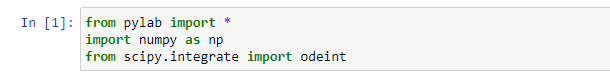
\includegraphics[width=11cm]{Img/1.PNG}
	\end{figure}

	Ahora necesitamos definir las constantes:
	\begin{figure}[h]
		\centering
		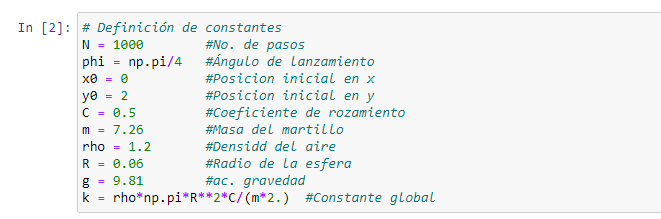
\includegraphics[width=11cm]{Img/2.PNG}
	\end{figure}

	Notemos que el coeficiente de rozamiento \texttt{C} será 0.75 para el flujo inestable oscilante, 0.5 para el flujo laminar y 0.0 para cuando no haya fuerza de fricción.\\
	En el método de Runge-Kutta para las EDO's requerimos de valores iniciales. En la siguiente función \texttt{cond\_ini}, dada una velocidad inicial $v_0$ se genera un arreglo de 4 valores con las condiciones iniciales de la siguiente forma: $[x_0, v_{0_x}, y_0, v_{0_y}]$. Esta función tendrá como parámetro una velocidad inicial $v_0$ y con ello calculará las velocidades $v_{0_x}=v_0\cos\phi$ y $v_{0_y}=v_0\sin\phi$ para arrojar el arreglo ya descrito.

\newpage
	\begin{figure}[h]
		\centering
		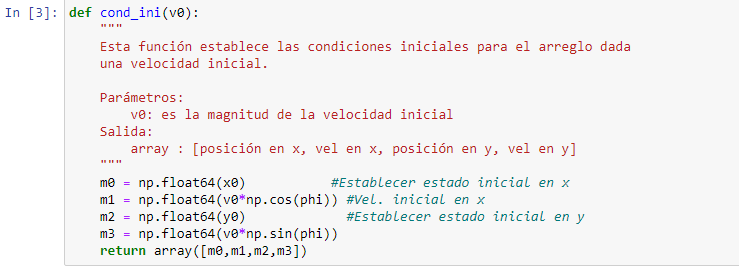
\includegraphics[width=10cm]{Img/3.PNG}
	\end{figure}

	Lo siguiente a realizar es una función que evalúe a las funciones $f^{(0)}, f^{(1)}, f^{(2)}$ y $f^{(3)}$ descritas en (\ref{ii}) y (\ref{iii})	para un punto $x,y$ en un intervalo de tiempo $t$.
	\begin{figure}[h]
		\centering
		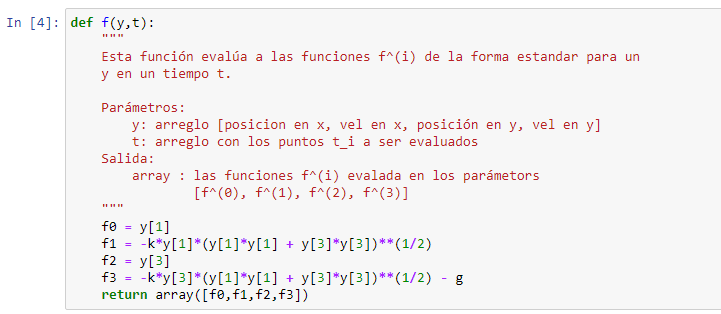
\includegraphics[width=10cm]{Img/4.PNG}
	\end{figure}

	Ahora nuestro propósito es generar una solución para una velocidad inicial $v_0$. La forma en como lo haremos será fijar el tiempo $t$ a 1 segundo y obtendremos la solución de 0 a 1 s. Luego a través de un ciclo \texttt{while} iremos aumentando el tiempo hasta generar la solución cuyo último valor para la posición en $y$ sea muy cercano al suelo. Es decir, que la solución final tendrá el momento en que el martillo se impacta en el suelo. Esto se observa en el siguiente algoritmo.
	\begin{figure}[h!]
		\centering
		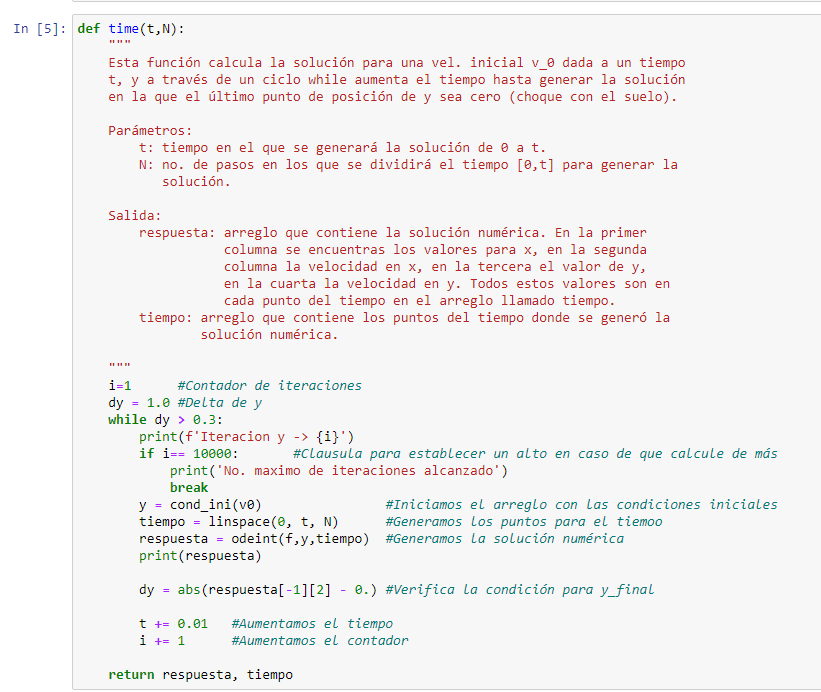
\includegraphics[width=11cm]{Img/5.PNG}
	\end{figure}
	
\newpage
	En esta última parte hay que tener cuidado con el criterio $dy > 0.3$ para que se rompa el ciclo \texttt{while} ya que es posible que la solución nunca cumpla con esto. Esa es la razón por la que se ha colocado un contador para un número máximo de iteraciones. En caso de alcanzar el número máximo de iteraciones, habría que hacer más grande el criterio colocado de 0.3.\\
	Lo siguiente a realizar para poder estimar la velocidad a la que se lanzó el martillo y con ello lograr una longitud de $\SI{86.74}{m}$, será usar otro ciclo \texttt{while} y al igual que en la función \texttt{time}, se generará la solución para la velocidad inicial $v_0$ hasta que el martillo impacte con el suelo y con ello evaluaremos la condición de que el $x$ final esté dentro de un intervalo aceptable para la longitud del récord. Esto se realiza en el siguiente algoritmo:
	\begin{figure}[h]
		\centering
		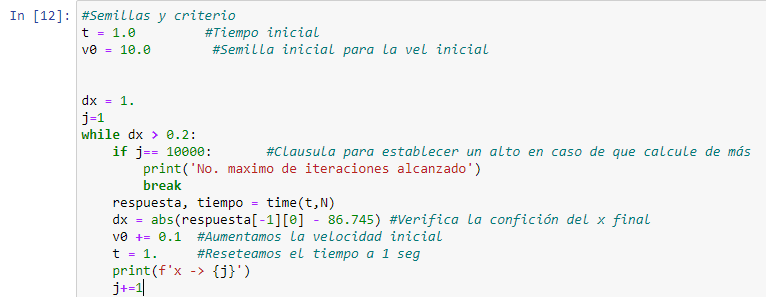
\includegraphics[width=11cm]{Img/6.PNG}
	\end{figure}
	
	Aquí hemos usado los valores semilla $v_0=\SI{10}{m/s}$ y $t=\SI{1}{s}$ para encontrar los que cumplen las condiciones establecidas. Cuando termine de generar la solución estas variables ($v_0,t$) guardaran la velocidad inicial y el tiempo del recorrido para lograr un alcance de $\SI{86.74}{m}$. Nuevamente hay que tener cuidado con el criterio $dx > 0.2$ para romper el ciclo \texttt{while}, en caso de no alcanzar el número máximo de iteraciones habría que aumentar el 0.2.\\\\
	
	Ya con esto es posible calcular la velocidad inicial a la que se realizó el lanzamiento de martillo para generar la longitud del récord para una fuerza de fricción. Para este inciso supondremos que el lanzamiento se hizo en condiciones muy ideales en las que no existió fricción. Para generar la solución sin fricción basta fijar $C_D=0.0$ en la definición de las constantes. Realizando esto e imprimiendo los resultados se obtiene:
		\begin{figure}[h]
		\centering
		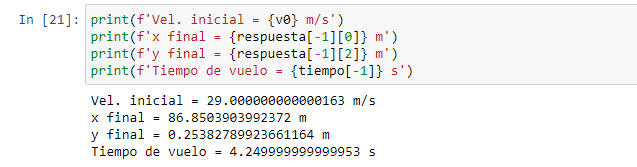
\includegraphics[width=10cm]{Img/7.PNG}
	\end{figure}
	
	Así hemos obtenido la solución para el lanzamiento sin fricción.Entonces la velocidad a la que se realizó en lanzamiento fue $v_0\approx\SI{29.0}{m/s}$ para el caso ideal sin fricción. Si graficamos la posición $y(t)$ contra el tiempo obtenemos:
\newpage
	\begin{figure}[h]
		\centering
		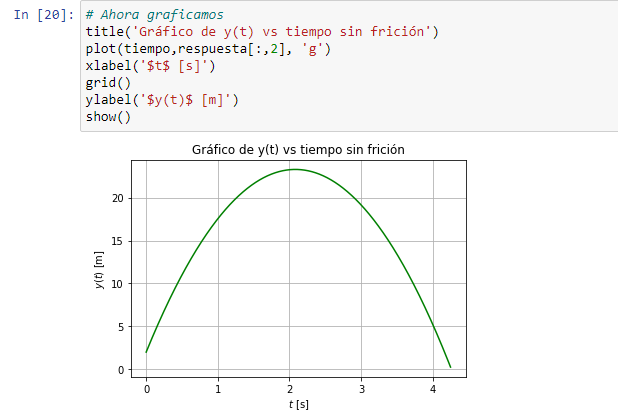
\includegraphics[width=12cm]{Img/8.PNG}
	\end{figure}
\hrule
	\begin{enumerate}
		\item [2.] Calcule y grafique la dependencia en el tiempo de la altitud del martillo y su trayectoria $y=y(t)$ en los tres régimenes:
		\begin{enumerate}
			\item [(a)] Sin fricción.
			\item [(b)] Flujo laminar.
			\item [(c)] Flujo inestable oscilante.
		\end{enumerate}
	\end{enumerate}
	\textit{Solución.}\\
	Para este inciso usaremos la velocidad inicial calculada en el ejercicio anterior. Es decir, $v_0\approx\SI{29.0}{m/s}$. A partir de esto generaremos la solución numérica de la trayectoria del martillo desde que es lanzado hasta que se impacta con el suelo. Esto para cada uno de los casos descritos. En el siguiente algoritmo generamos las soluciones numéricas para cada uno de los casos.
	\begin{figure}[h!]
		\centering
		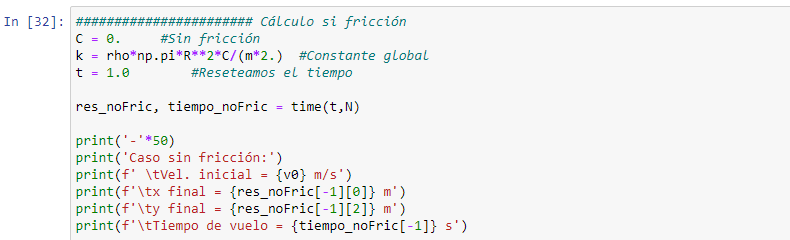
\includegraphics[width=12cm]{Img/9.1.PNG}
	\end{figure}
\newpage
	\begin{figure}[h!]
		\centering
		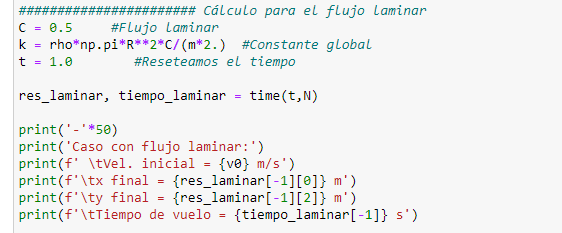
\includegraphics[width=10cm]{Img/9.2.PNG}
	\end{figure}
	\begin{figure}[h!]
		\centering
		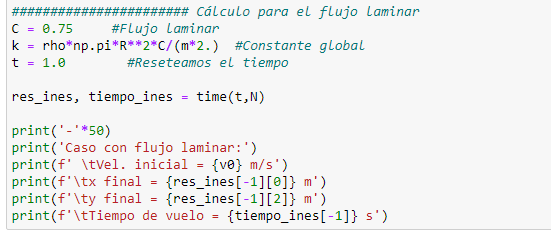
\includegraphics[width=9.6cm]{Img/9.3.PNG}
	\end{figure}
	
	Estas soluciones nos producen los siguientes resultados:
	\begin{figure}[h!]
		\centering
		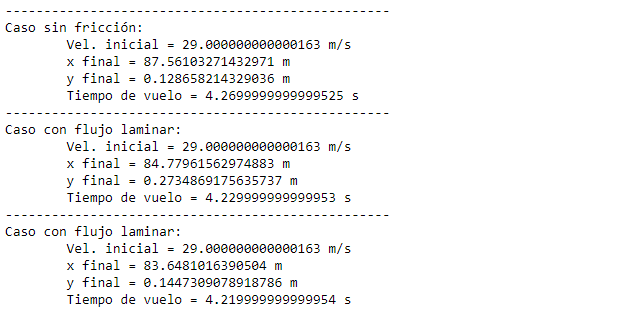
\includegraphics[width=11cm]{Img/10.PNG}
	\end{figure}
	
	Se puede observar como al agregar fricción la longitud $x$ recorrida es menor y a su vez el tiempo de vuelo también disminuye. \\
	Ahora veamos gráficamente como difieren las soluciones. En el siguiente algoritmo se generan dos subgráficas: la primera muestra la superposición de los tres casos de $y(t)$ vs $t$ para la velocidad $v_0$ obtenida en el ejercicio 1. La segunda subgráfica contiene la superposición de $y(t)$ vs $x(t)$ para los tres casos. 
\newpage
	\begin{figure}[h!]
		\centering
		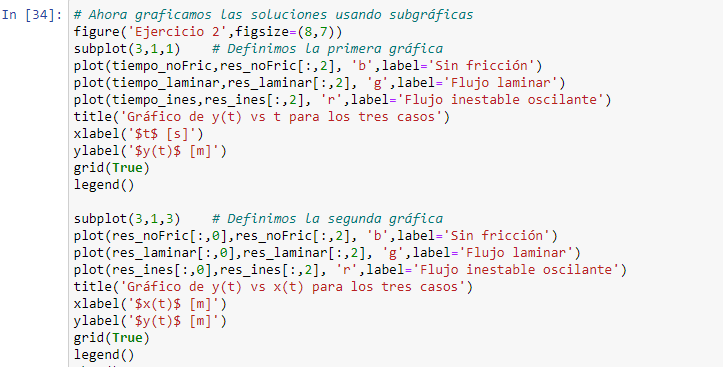
\includegraphics[width=12cm]{Img/11.PNG}
	\end{figure}
	Esto nos produce los siguientes dos subgráficos:
	\begin{figure}[h!]
		\centering
		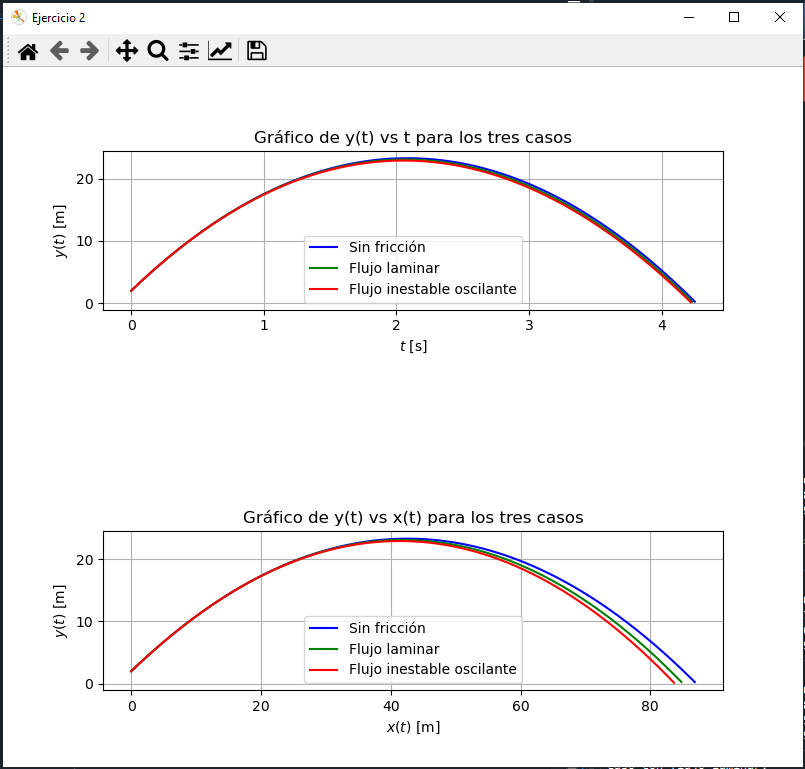
\includegraphics[width=12cm]{Img/12.PNG}
	\end{figure}

	En el primer subgráfico se puede ver que el tiempo de recorrido es casi el mismo en los tres casos. Sin embargo, en el segundo gráfico se observa que existe una diferencia significativa en la longitud $x$ recorrida. Como es de esperarse, al ser mayor la fuerza de fricción es menor la longitud total recorrida. En el siguiente ejercicio obtendremos la diferencia de longitudes.
\hrule
\newpage
	\begin{enumerate}
		\item [3.] En el inciso anterior, estime la cantidad en que es influenciada la distancia del lanzamiento por la fricción. 
	\end{enumerate}
	\textit{Solución.}\\
	Este inciso es muy simple. Debido a la forma en como hemos realizado nuestro programa, basta comparar la última entrada de la primer columna de los arreglos \texttt{res\_noFric}, \texttt{res\_laminar} y \texttt{res\_ines}. En esa posición se encuentra la posición $x$ donde el martillo chocó con el suelo al final del recorrido. Tomaremos el caso sin fricción como el que describe el lanzamiento de martillo, de esa forma obtendremos la diferencia de longitud para el flujo laminar y flujo inestable oscilante con respecto al caso sin fricción. Esto se hace en el siguiente algoritmo con su correspondiente resultado:
	 \begin{figure}[h!]
	 	\centering
	 	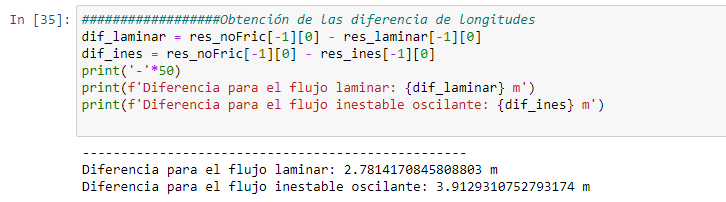
\includegraphics[width=14cm]{Img/13.PNG}
	 \end{figure}
 
 	Por lo que en presencia de flujo laminar el martillo llegará aproximadamente 2.78 m antes del récord y en presencia de flujo inestable oscilante llegará 3.91 m antes.
\end{document}